\documentclass[]{article}
\usepackage{lmodern}
\usepackage{amssymb,amsmath}
\usepackage{ifxetex,ifluatex}
\usepackage{fixltx2e} % provides \textsubscript
\ifnum 0\ifxetex 1\fi\ifluatex 1\fi=0 % if pdftex
  \usepackage[T1]{fontenc}
  \usepackage[utf8]{inputenc}
\else % if luatex or xelatex
  \ifxetex
    \usepackage{mathspec}
  \else
    \usepackage{fontspec}
  \fi
  \defaultfontfeatures{Ligatures=TeX,Scale=MatchLowercase}
\fi
% use upquote if available, for straight quotes in verbatim environments
\IfFileExists{upquote.sty}{\usepackage{upquote}}{}
% use microtype if available
\IfFileExists{microtype.sty}{%
\usepackage{microtype}
\UseMicrotypeSet[protrusion]{basicmath} % disable protrusion for tt fonts
}{}
\usepackage[margin=1in]{geometry}
\usepackage{hyperref}
\hypersetup{unicode=true,
            pdftitle={MAP 531: Homework},
            pdfauthor={Paul-Antoine GIRARD \& Adrien TOULOUSE},
            pdfborder={0 0 0},
            breaklinks=true}
\urlstyle{same}  % don't use monospace font for urls
\usepackage{color}
\usepackage{fancyvrb}
\newcommand{\VerbBar}{|}
\newcommand{\VERB}{\Verb[commandchars=\\\{\}]}
\DefineVerbatimEnvironment{Highlighting}{Verbatim}{commandchars=\\\{\}}
% Add ',fontsize=\small' for more characters per line
\usepackage{framed}
\definecolor{shadecolor}{RGB}{248,248,248}
\newenvironment{Shaded}{\begin{snugshade}}{\end{snugshade}}
\newcommand{\AlertTok}[1]{\textcolor[rgb]{0.94,0.16,0.16}{#1}}
\newcommand{\AnnotationTok}[1]{\textcolor[rgb]{0.56,0.35,0.01}{\textbf{\textit{#1}}}}
\newcommand{\AttributeTok}[1]{\textcolor[rgb]{0.77,0.63,0.00}{#1}}
\newcommand{\BaseNTok}[1]{\textcolor[rgb]{0.00,0.00,0.81}{#1}}
\newcommand{\BuiltInTok}[1]{#1}
\newcommand{\CharTok}[1]{\textcolor[rgb]{0.31,0.60,0.02}{#1}}
\newcommand{\CommentTok}[1]{\textcolor[rgb]{0.56,0.35,0.01}{\textit{#1}}}
\newcommand{\CommentVarTok}[1]{\textcolor[rgb]{0.56,0.35,0.01}{\textbf{\textit{#1}}}}
\newcommand{\ConstantTok}[1]{\textcolor[rgb]{0.00,0.00,0.00}{#1}}
\newcommand{\ControlFlowTok}[1]{\textcolor[rgb]{0.13,0.29,0.53}{\textbf{#1}}}
\newcommand{\DataTypeTok}[1]{\textcolor[rgb]{0.13,0.29,0.53}{#1}}
\newcommand{\DecValTok}[1]{\textcolor[rgb]{0.00,0.00,0.81}{#1}}
\newcommand{\DocumentationTok}[1]{\textcolor[rgb]{0.56,0.35,0.01}{\textbf{\textit{#1}}}}
\newcommand{\ErrorTok}[1]{\textcolor[rgb]{0.64,0.00,0.00}{\textbf{#1}}}
\newcommand{\ExtensionTok}[1]{#1}
\newcommand{\FloatTok}[1]{\textcolor[rgb]{0.00,0.00,0.81}{#1}}
\newcommand{\FunctionTok}[1]{\textcolor[rgb]{0.00,0.00,0.00}{#1}}
\newcommand{\ImportTok}[1]{#1}
\newcommand{\InformationTok}[1]{\textcolor[rgb]{0.56,0.35,0.01}{\textbf{\textit{#1}}}}
\newcommand{\KeywordTok}[1]{\textcolor[rgb]{0.13,0.29,0.53}{\textbf{#1}}}
\newcommand{\NormalTok}[1]{#1}
\newcommand{\OperatorTok}[1]{\textcolor[rgb]{0.81,0.36,0.00}{\textbf{#1}}}
\newcommand{\OtherTok}[1]{\textcolor[rgb]{0.56,0.35,0.01}{#1}}
\newcommand{\PreprocessorTok}[1]{\textcolor[rgb]{0.56,0.35,0.01}{\textit{#1}}}
\newcommand{\RegionMarkerTok}[1]{#1}
\newcommand{\SpecialCharTok}[1]{\textcolor[rgb]{0.00,0.00,0.00}{#1}}
\newcommand{\SpecialStringTok}[1]{\textcolor[rgb]{0.31,0.60,0.02}{#1}}
\newcommand{\StringTok}[1]{\textcolor[rgb]{0.31,0.60,0.02}{#1}}
\newcommand{\VariableTok}[1]{\textcolor[rgb]{0.00,0.00,0.00}{#1}}
\newcommand{\VerbatimStringTok}[1]{\textcolor[rgb]{0.31,0.60,0.02}{#1}}
\newcommand{\WarningTok}[1]{\textcolor[rgb]{0.56,0.35,0.01}{\textbf{\textit{#1}}}}
\usepackage{graphicx,grffile}
\makeatletter
\def\maxwidth{\ifdim\Gin@nat@width>\linewidth\linewidth\else\Gin@nat@width\fi}
\def\maxheight{\ifdim\Gin@nat@height>\textheight\textheight\else\Gin@nat@height\fi}
\makeatother
% Scale images if necessary, so that they will not overflow the page
% margins by default, and it is still possible to overwrite the defaults
% using explicit options in \includegraphics[width, height, ...]{}
\setkeys{Gin}{width=\maxwidth,height=\maxheight,keepaspectratio}
\IfFileExists{parskip.sty}{%
\usepackage{parskip}
}{% else
\setlength{\parindent}{0pt}
\setlength{\parskip}{6pt plus 2pt minus 1pt}
}
\setlength{\emergencystretch}{3em}  % prevent overfull lines
\providecommand{\tightlist}{%
  \setlength{\itemsep}{0pt}\setlength{\parskip}{0pt}}
\setcounter{secnumdepth}{0}
% Redefines (sub)paragraphs to behave more like sections
\ifx\paragraph\undefined\else
\let\oldparagraph\paragraph
\renewcommand{\paragraph}[1]{\oldparagraph{#1}\mbox{}}
\fi
\ifx\subparagraph\undefined\else
\let\oldsubparagraph\subparagraph
\renewcommand{\subparagraph}[1]{\oldsubparagraph{#1}\mbox{}}
\fi

%%% Use protect on footnotes to avoid problems with footnotes in titles
\let\rmarkdownfootnote\footnote%
\def\footnote{\protect\rmarkdownfootnote}

%%% Change title format to be more compact
\usepackage{titling}

% Create subtitle command for use in maketitle
\providecommand{\subtitle}[1]{
  \posttitle{
    \begin{center}\large#1\end{center}
    }
}

\setlength{\droptitle}{-2em}

  \title{MAP 531: Homework}
    \pretitle{\vspace{\droptitle}\centering\huge}
  \posttitle{\par}
    \author{Paul-Antoine GIRARD \& Adrien TOULOUSE}
    \preauthor{\centering\large\emph}
  \postauthor{\par}
    \date{}
    \predate{}\postdate{}
  
\usepackage{dsfont}

\begin{document}
\maketitle

You are asked to provided answers to all these exercises as both Rmd and
pdf files. The two files should be uploaded on Moodle on the 15th of
November (23h59 Paris time). This homework should be done by groups of
2. Only one submission per group on moodle, with both names indicated in
the file. This homework is composed of 2 independent problems. Some of
the questions are a bit more technical: they are marked by a * and are
optional.

\hypertarget{problem-1-estimating-parameters-of-a-poisson-distribution-to-model-the-number-of-goals-scored-in-football}{%
\section{Problem 1: Estimating parameters of a Poisson distribution to
model the number of goals scored in
football}\label{problem-1-estimating-parameters-of-a-poisson-distribution-to-model-the-number-of-goals-scored-in-football}}

We recall that the Poisson distribution with parameter \(\theta > 0\)
has a pdf given by (\(p(\theta, k), k \in \mathbb{N})\) w.r.t the
counting measure on \(\mathbb{N}\):
\(p(\theta, k) = e^{-\theta} \frac{\theta^k}{k!}\)

\hypertarget{question-1-is-it-a-discrete-or-continuous-distribution-can-you-give-3-examples-of-phenomenons-that-could-be-modeled-by-such-a-distribution-in-statistics}{%
\subsection{Question 1: Is it a discrete or continuous distribution? Can
you give 3 examples of phenomenons that could be modeled by such a
distribution in
statistics?}\label{question-1-is-it-a-discrete-or-continuous-distribution-can-you-give-3-examples-of-phenomenons-that-could-be-modeled-by-such-a-distribution-in-statistics}}

The poisson distribution is a discrete distribution since it has a
countable number of possible values (\(\mathbb{N}\)).

In statistics, we use this distribution to compute the probability of a
given number of (rare) events in a time period or the probability of a
discrete waiting time until the next event (eg. number of minutes).

For example a poisson distribution can model:

\begin{itemsize}
\item The number of patients arriving in an emergency room between 9 and 10am.
\item The number of minutes we wait a bus at the bus stop.
\item In quality control, the number of manufacturing defect.
\end{itemsize}

\hypertarget{question-2-compute-the-mean-and-the-variance-of-this-distribution.}{%
\subsection{Question 2: Compute the mean and the variance of this
distribution.}\label{question-2-compute-the-mean-and-the-variance-of-this-distribution.}}

We assume that \(\mathbb{X}\) follows a Poisson distribution with
parameter \(\theta > 0\).
\(\mathbb{E}[\mathbb{X}] = \sum_{i=0}^{\infty} (i * p(\theta, i))\)
\(= \sum_{i=0}^{\infty} (i*e^{-\theta} \frac{\theta^{i}}{i!})\)
\(= \theta * e^{-\theta}\sum_{i=1}^{\infty} (\frac{\theta^{i-1}}{(i-1)!})\)

\(= \theta * e^{-\theta}\sum_{i=0}^{\infty} (\frac{\theta^{i}}{i!})\)
\(= \theta * e^{-\theta} * e^{\theta}\) \(= \theta\)

\(\mathbb{E}[\mathbb{X}^2] = \sum_{i=0}^{\infty} (i^2 * p(\theta, i))\)
\(= \sum_{i=0}^{\infty} (i^2*e^{-\theta} \frac{\theta^{i}}{i!})\)
\(= \theta * e^{-\theta}\sum_{i=1}^{\infty} (i\frac{\theta^{i-1}}{(i-1)!})\)
\newline
\(= \theta * e^{-\theta}\sum_{i=0}^{\infty} ((i+1)\frac{\theta^{i}}{i!})\)
\(= \theta * e^{-\theta}[\sum_{i=0}^{\infty} (i\frac{\theta^{i}}{i!}) + \sum_{i=0}^{\infty} (\frac{\theta^{i}}{i!})]\)
\newline \(= \theta * e^{-\theta}[\theta * e^{\theta} + e^{\theta}]\)
\(= \theta (\theta + 1)\)

\hypertarget{question-3-what-are-our-observations-what-distribution-do-they-follow-write-the-corresponding-statistical-model.-what-parameter-are-we-trying-to-estimate}{%
\subsection{Question 3: What are our observations? What distribution do
they follow? Write the corresponding statistical model. What parameter
are we trying to
estimate?}\label{question-3-what-are-our-observations-what-distribution-do-they-follow-write-the-corresponding-statistical-model.-what-parameter-are-we-trying-to-estimate}}

We are provided with n independent observations of a Poisson random
variable of parameter \(\theta > 0\). The corresponding statistical
model is \(\mathbb{M} = \{p(.\mid \theta),\ \theta \in\Theta \}\) We are
trying to estimate \(\theta\).

\hypertarget{question-4-what-is-the-likelihood-function-compute-the-maximum-likelihood-estimator.}{%
\subsection{Question 4: What is the likelihood function? Compute the
Maximum Likelihood
Estimator.}\label{question-4-what-is-the-likelihood-function-compute-the-maximum-likelihood-estimator.}}

The likelihood function is the function on \(\theta\) that makes our n
observations most likely.

\(l(\theta) = \prod_{k=1}^{\infty} p(\theta,k) = \prod_{k=1}^{\infty} e^{-\theta} \frac{\theta^{x_{k}}}{x_{k}!}\)
\(L(\theta) = log(l(\theta)) = -n\theta + log(\theta)\sum_{k=1}^{\infty}x_{k}-\sum_{k=1}^{\infty}log(x_{k}!)\)

By derivating with respect to \(\theta\) :

\hypertarget{question-5-prove-that-nux3b8ux2c6ml-ux3b8-converges-in-distribution-as-n-.}{%
\subsection{Question 5: Prove that √n(θˆML − θ) converges in
distribution as n →
∞.}\label{question-5-prove-that-nux3b8ux2c6ml-ux3b8-converges-in-distribution-as-n-.}}

The central limit theorem gives us that
\(\sqrt{n}(\hat\theta_{MLE}-\theta)\) converges towards a Gaussian
\(N(0,\theta)\)

\hypertarget{question-6}{%
\subsection{Question 6:}\label{question-6}}

By continuous mapping, \(\sqrt{\hat\theta_{MLE}}\) converges in
probability towards \(\sqrt{\theta}\). Then, by Slutsky's theorem, we
have that
\(\sqrt{n}\frac{(\hat\theta_{MLE}-\theta)}{\sqrt{\hat\theta_{MLE}}}\)
converges in law towards a gaussian \(N(0,1)\).

Let's check this result in R by simulating 1000 times our random
variable
\(\sqrt{n}\frac{(\hat\theta_{MLE}-\theta)}{\sqrt{\hat\theta_{MLE}}}\)
with a sample size of 100:

\begin{Shaded}
\begin{Highlighting}[]
\NormalTok{Nattempts =}\StringTok{ }\DecValTok{1000}
\NormalTok{nsample =}\StringTok{ }\DecValTok{100}
\ControlFlowTok{for}\NormalTok{ (i }\ControlFlowTok{in} \DecValTok{1}\OperatorTok{:}\NormalTok{Nattempts)  }\CommentTok{# can be written without the for loop (nicer) !}
\NormalTok{\{poisson_sample =}\StringTok{ }\KeywordTok{rpois}\NormalTok{(nsample, }\DataTypeTok{lambda =} \DecValTok{3}\NormalTok{)}
\NormalTok{  sample =}\StringTok{ }\KeywordTok{sqrt}\NormalTok{(nsample) }\OperatorTok{*}\StringTok{ }\NormalTok{(}\KeywordTok{mean}\NormalTok{(poisson_sample) }\OperatorTok{-}\StringTok{ }\NormalTok{poisson_sample) }\OperatorTok{/}\StringTok{ }\KeywordTok{sqrt}\NormalTok{(}\KeywordTok{mean}\NormalTok{(poisson_sample))}
\NormalTok{\}  }

\KeywordTok{hist}\NormalTok{(sample)}
\end{Highlighting}
\end{Shaded}

\includegraphics{homework_files/figure-latex/unnamed-chunk-1-1.pdf}

\begin{Shaded}
\begin{Highlighting}[]
\KeywordTok{qqnorm}\NormalTok{(sample)}
\KeywordTok{qqline}\NormalTok{(sample)}
\end{Highlighting}
\end{Shaded}

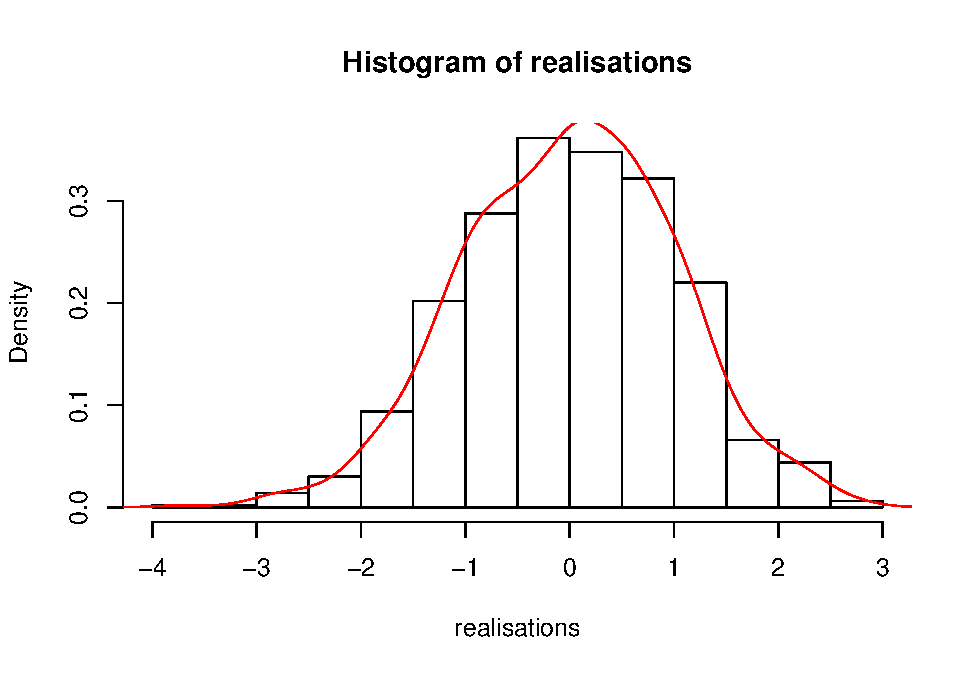
\includegraphics{homework_files/figure-latex/unnamed-chunk-2-1.pdf}

\hypertarget{question-7}{%
\subsection{Question 7:}\label{question-7}}

Let \(Z_n\) be our random variable, so that \$ Z\_n =
\sqrt{n}\frac{(\hat\theta_{MLE}-\theta)}{\sqrt{\hat\theta_{MLE}}}\$

\(\begin{equation} P(-z_{1-\alpha/2} ≤ Z_n ≤ z_{1-\alpha/2}) = 1- \alpha \iff P(-z_{1-\alpha/2} \sqrt{\frac{\hat\theta_{MLE}}{n}}≤ \hat\theta_{MLE} - \theta ≤ z_{1-\alpha/2}\sqrt{\frac{\hat\theta_{MLE}}{n}})= 1- \alpha \end{equation}\)

For \(\alpha \in (0, 1)\), an asymptotic confidence interval for
\(\theta\) of level \(\alpha\) is therefore :

\([\hat\theta_{MLE}-z_{1-\alpha/2}\frac{\sqrt{\hat\theta_{MLE}}}{\sqrt{n}};\hat\theta_{MLE}+z_{1-\alpha/2}\frac{\sqrt{\hat\theta_{MLE}}}{\sqrt{n}} ]\)


\end{document}
